\chapter{Pruebas de software}
\label{chap:chapter3}


El presente capítulo tiene como objetivo validar el correcto funcionamiento del sistema multiagente conversacional desarrollado para interpretar y contextualizar los datos no estructurados del transporte marítimo recogidos en el \textit{Diario de la Marina}. A través de un conjunto de pruebas cuidadosamente diseñadas, se evalúa si el sistema cumple con los requisitos funcionales y no funcionales previamente definidos, así como con los criterios de calidad establecidos por el modelo ISO/IEC 25010.

Para ello, se ejecutan pruebas unitarias, de integración y funcionales sobre los distintos componentes del sistema, prestando especial atención al comportamiento del microservicio de inteligencia artificial encargado del procesamiento conversacional. Asimismo, se emplean métricas como el tiempo de respuesta, la coherencia semántica de las respuestas generadas y la capacidad de recuperación de información relevante.

Además, se incluyen pruebas empíricas orientadas a medir la usabilidad desde la perspectiva del usuario final, validando si la interfaz permite una interacción fluida y si el sistema entrega respuestas precisas y contextualizadas ante consultas históricas reales.

\section{Pruebas de software}

Las pruebas tratan de demostrar que un programa hace lo que se intenta que haga, así como descubrir defectos en el programa antes de usarlo. Al probar el software, se ejecuta un programa con datos artificiales. Hay que verificar los resultados de la prueba que se opera para buscar errores, anomalías o información de atributos no funcionales del
programa~\cite{sommerville2011software}. A fin de encontrar los errores del sistema y garantizar un nivel aceptable de calidad y confianza, se realizaron pruebas de software, de caja negra, tanto manuales como automatizadas, haciendo uso de las principales técnicas existentes, y aprovechando las pruebas automatizadas, apoyándose en la estrategia de pruebas recomendada por el CMS, Desarrollo dirigido por pruebas (\textit{Test Driver Development}, por sus siglas en inglés TDD).

\section{Estrategia de pruebas}

La elaboración de todo producto de software implica la posibilidad de introducción de errores que provocan fallos en el sistema desarrollado. Por este motivo debe existir una vía para garantizar su calidad y correcto funcionamiento. La realización de pruebas es una actividad que permite verificar el producto bajo ciertas condiciones y en base a los requerimientos identificados para la construcción del mismo, los resultados son observados y registrados para su corrección.

\begin{longtable}{|p{2.5cm}|p{3cm}|p{3cm}|p{6cm}|}
	\caption{Estrategia de pruebas} \label{tab:plan-pruebas} \\
	\hline
	\textbf{Tipos de pruebas} & \textbf{Método} & \textbf{Herramienta} & \textbf{Alcance} \\
	\hline
	\endfirsthead
	
	\hline
	\textbf{Prueba} & \textbf{Método} & \textbf{Herramienta} & \textbf{Alcance} \\
	\hline
	\endhead
	
	Unitaria & Caja blanca aplicando la técnica del camino básico & Módulo TestCase de Django para la realización de pruebas automatizadas & Se automatizarán pruebas para las unidades de código separadas por requisitos funcionales. \\
	\hline
	Funcional & Caja negra aplicando la técnica de particiones equivalentes & SeleniumIDE & Se probará el funcionamiento del 100\% de los requisitos. \\
	\hline
	Rendimiento & Pruebas de carga y estrés & Locust & Se aplicará sobre un entorno de pruebas con prestaciones similares a las de despliegue establecidas en los requisitos no funcionales. Se probará la aplicación con 20 usuarios concurrentes buscando tiempos de respuesta menores a 5 segundos. \\
	\hline
	Seguridad &  & \textit{Acunetix Web Vulnerability Scanner} 9.5 & Se aplicará para detectar vulnerabilidades:
	\begin{itemize}[left=0pt]
		\item Inyección SQL
		\item Programación Cross-Site (XSS)
		\item Ataques de fuerza bruta a las credenciales
		\item Redirecciones y reenvíos no validados
	\end{itemize} \\
	\hline
\end{longtable}

\section{Pruebas unitarias}

Las pruebas unitarias son una técnica de desarrollo de software que consiste en verificar el correcto funcionamiento de las unidades individuales más pequeñas de un programa, como funciones o métodos. Su objetivo principal es asegurar que cada parte del código funcione según lo esperado, facilitando la detección de errores en etapas tempranas del desarrollo. Las pruebas unitarias son una parte esencial de las metodologías ágiles, ya que permiten mantener la calidad del software a lo largo del proceso de desarrollo.Estas pruebas las ejecuta el desarrollador, cada vez que va probando fragmentos de código
o scripts para ver si todo funciona como se desea. Proporcionan un contrato escrito, que el fragmento de código debe satisfacer. El método utilizado para realizar este tipo de prueba se denomina caja
blanca~\cite{sommerville2011software}.

\subsection{Método de caja blanca}

Las pruebas de caja blanca intentan garantizar que:

\begin{itemize}
	\item Se ejecutan al menos una vez todos los caminos independientes de cada requisito funcional.
	\item Se utilizan las decisiones en su parte verdadera y en su parte falsa.
	\item Se ejecuten todos los bucles en sus límites.
	\item Se utilizan todas las estructuras de datos internas.
\end{itemize}

Para la realización de las pruebas unitarias, se le aplicó la técnica de prueba del camino básico a las unidades
código que responden a funcionalidades críticas del software, lo cual permitió generar el grafo de flujo,
calcular la Complejidad Ciclomática (CC) para determinar los caminos linealmente independientes y el
número mínimo de escenarios de los casos de prueba para forzar la ejecución de cada camino del conjunto
básico.
Luego en apoyo a las pruebas se usó el módulo \textit{TestCase} que ofrece \textit{Django REST Framework}, para la automatización de las pruebas unitarias. Con él se probó cada módulo desarrollado, y gracias a la aplicación de la
técnica de camino básico, en aquellas funcionalidades críticas, se pudieron automatizar pruebas para cada
uno de los escenarios o caminos posibles, garantizando probar todo el código en cuestión.

Entre los elementos de código que fueron probadas se encuentra el referente al método \textit{post} de la clase
\textit{Message\_Create\_AV}, que se encarga de crear los mensajes tanto del usario como de las respuestas del sistema al usuario en una conversación asociada.

\begin{table}[h]
	\centering
	\caption{Cálculo de la complejidad ciclomática del método \textit{post} de la clase \textit{Message\_Create\_AV}}
	\label{tab:complejidad-ciclomatica}
	\begin{tabular}{|c|}
		\hline
		Método \\
		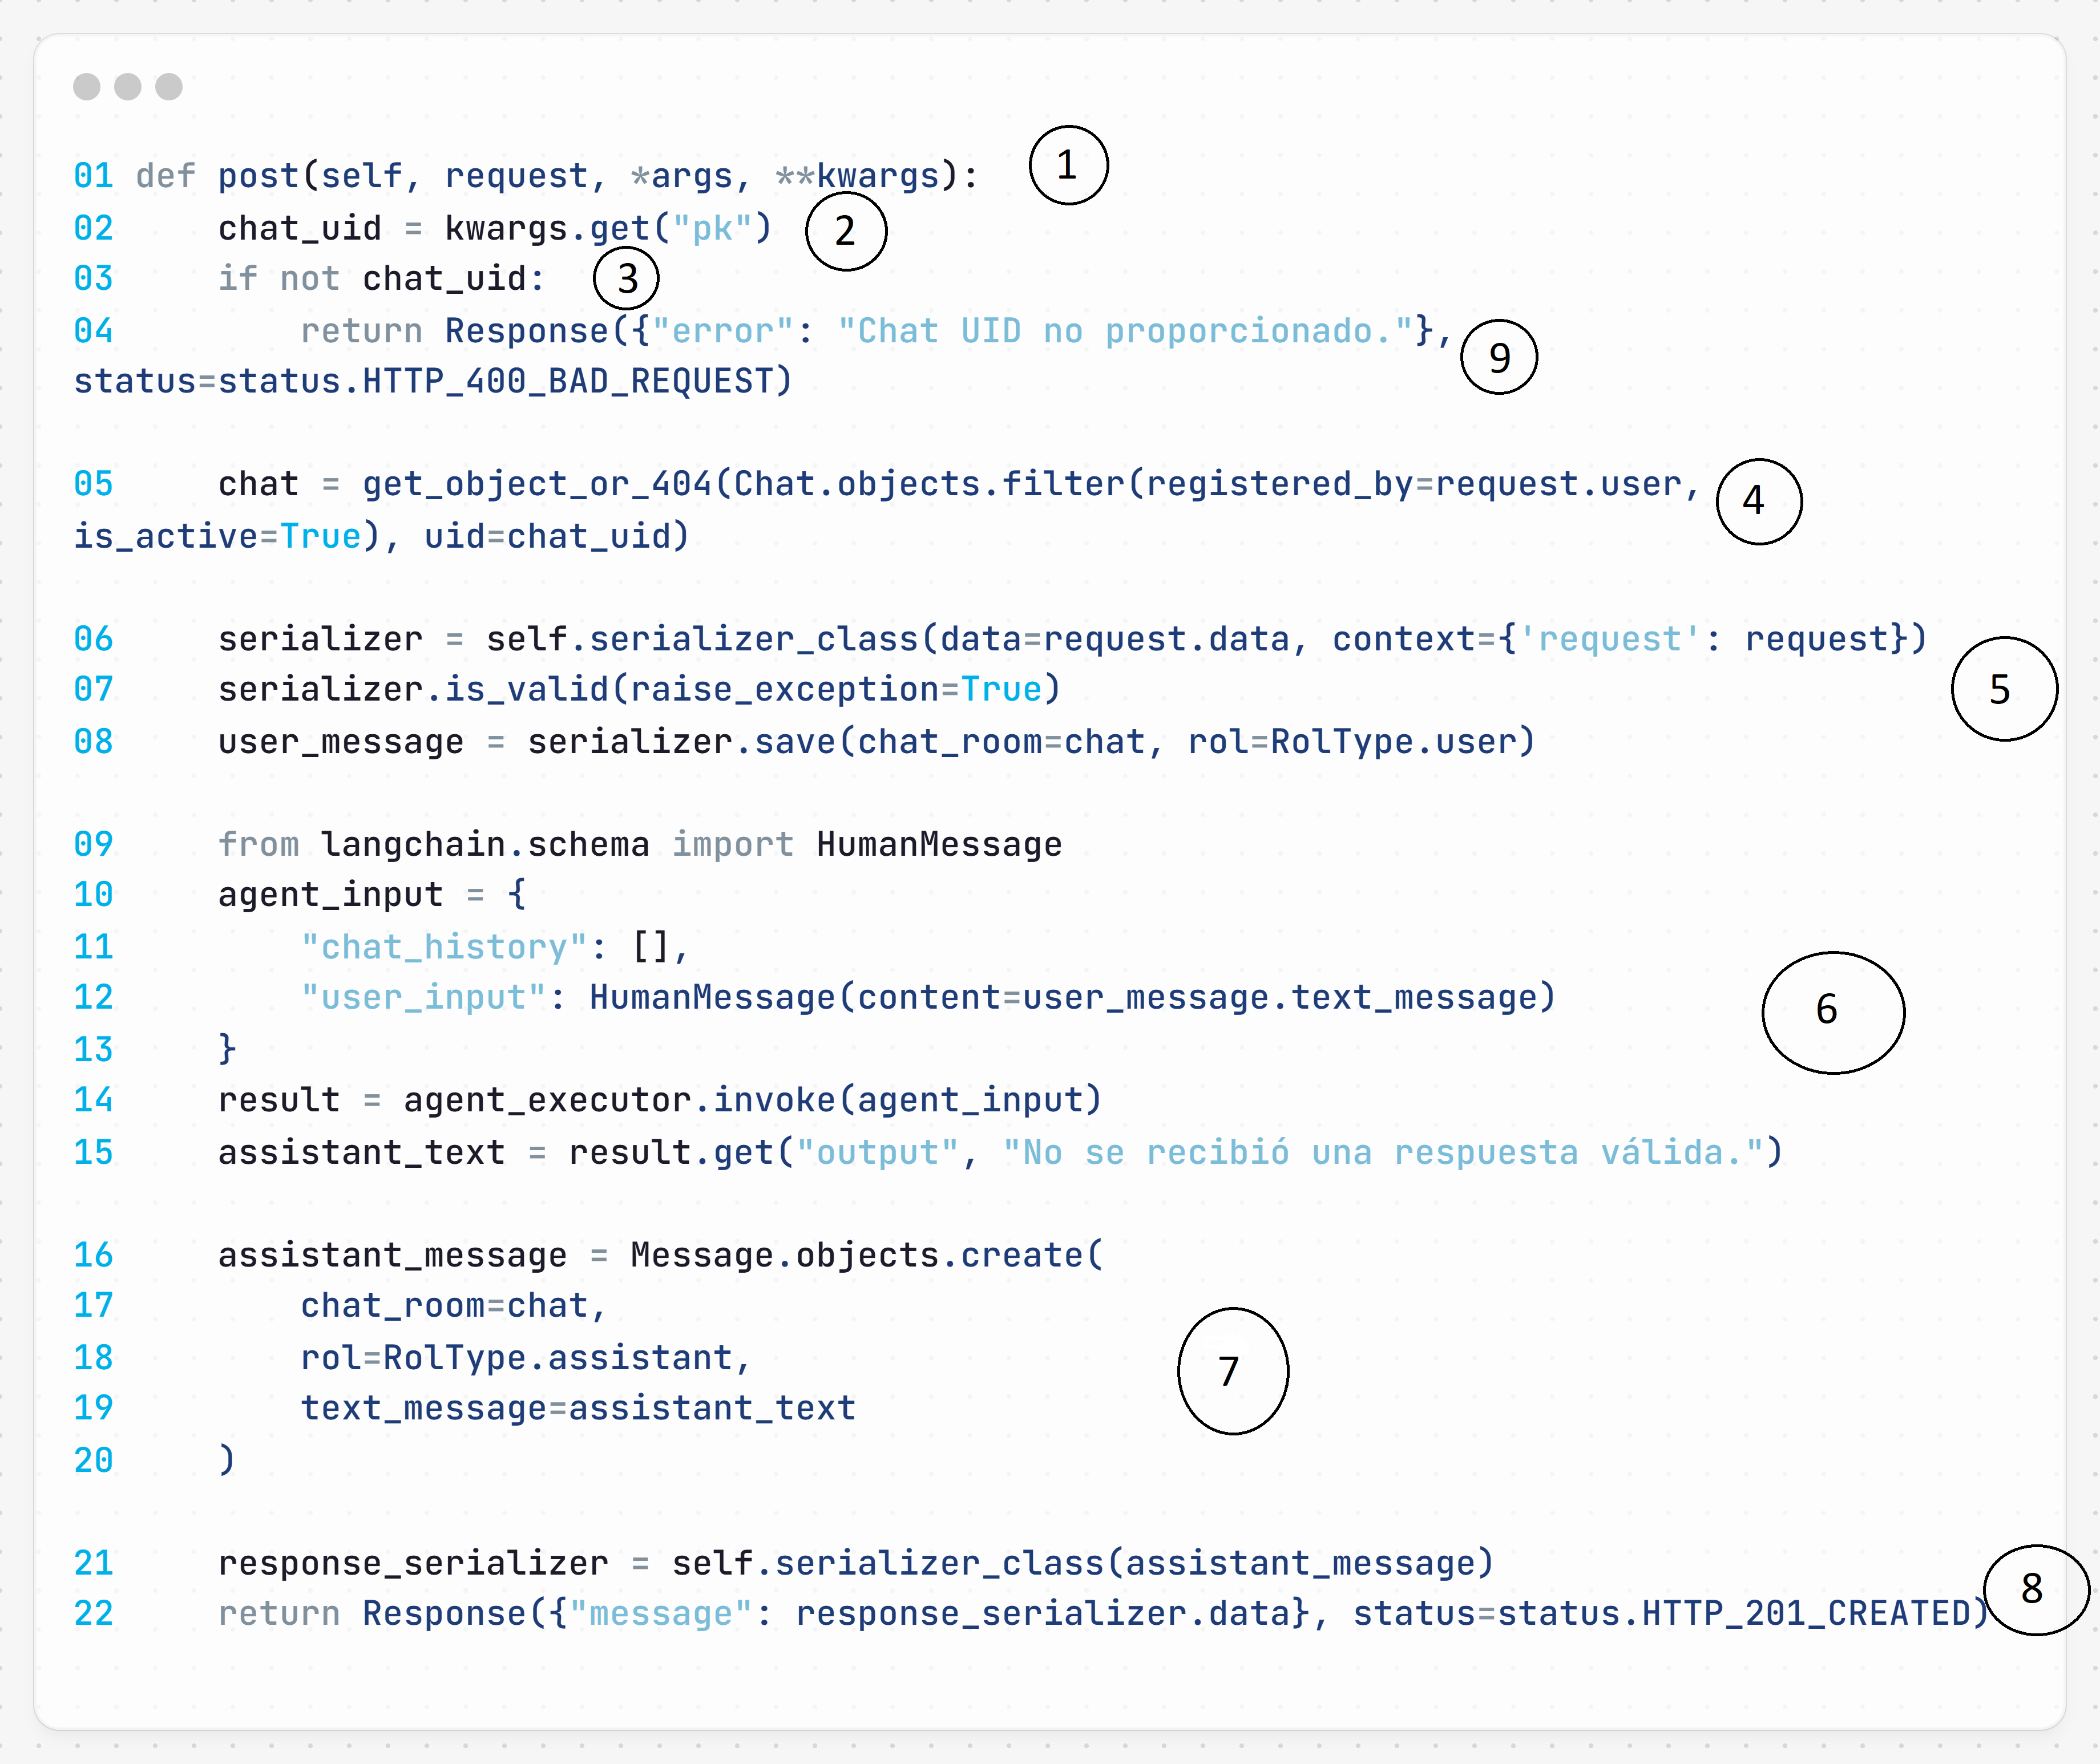
\includegraphics[width=0.4\linewidth]{images/postCreateMessage.png} \\
		\hline
		Grafo \\
		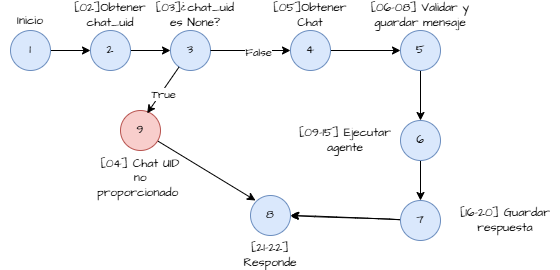
\includegraphics[width=0.4\linewidth]{images/postMessage.png} \\
		\hline
	\end{tabular}
\end{table}

\begin{table}[H]
	\centering
	\caption{Cálculo de la complejidad ciclomática del método \texttt{post} de la clase \texttt{Message\_Create\_AV}}
	\label{tab:complejidad-ciclomatica2}
	\renewcommand{\arraystretch}{1.5}
	\begin{tabular}{|>{\bfseries}m{5cm}|m{4cm}|m{4cm}|}
		\hline
		Complejidad Ciclomática: & \( V(G) = A - N + 2 \) & \( V(G) = P + 1 \) \\
		\hline
		\( V(G) = \# \textit{ de regiones} \) & \( V(G) = 9 - 9 + 2 \) & \( V(G) = 1 + 1 \) \\
		\hline
		\( V(G) = 2 \) & \( V(G) = 2 \) & \( V(G) = 2 \) \\
		\hline
	\end{tabular}
\end{table}

Luego de la determinación de los nodos y flujos de control del código se obtuvo el grafo de flujo y se calculó la complejidad ciclomática del algoritmo.
Como resultado se obtuvo que la complejidad ciclomática es igual a 2, lo que significa que existen dos posibles caminos
linealmente independientes y hay que diseñar un mínimo de dos casos de prueba para el algoritmo. La Tabla \ref{tab:caminos-grafos2} muestra los caminos existentes.

\begin{table}[h]
	\centering
	\caption{Caminos del grafo de flujo (Fuente: Elaboración propia).}
	\label{tab:caminos-grafos2}
	\begin{tabular}{|>{\bfseries}m{5cm}|m{4cm}|m{4cm}|}
		\hline
		\textbf{No.} & \textbf{Camino} \\ \hline
		1            & 1, 2, 3, 9      \\ \hline
		2            & 1, 2, 3, 4, 5, 6, 7, 8   \\ \hline
	\end{tabular}
\end{table}

Los casos de prueba para las pruebas de caja blanca por la técnica de camino básico se ejecutan por cada
camino independiente que se determine en un algoritmo específico. A continuación, se muestra el caso de
prueba para el camino básico independiente 2 del algoritmo.

\begin{longtable}{|p{4cm}|p{11cm}|}
	\caption{Caso de Prueba para el camino básico 1 (Fuente: Elaboración propia).}
	\label{tab:caminos-grafo}\\
	\hline
	\textbf{Proceso} &  \\ \hline
	\textbf{Caso de prueba} & Recibir consulta . Escenario 1.1 \\ \hline
	\textbf{Camino independiente} & 1, 2, 3, 9 \\ \hline
	\textbf{Entradas} &
	\begin{itemize}
		\item \textbf{Consulta}: Lista los barcos que entraron al puerto de la Habana en 1851.
		\item \textbf{uid\_sala\_de\_chat:} Con valor nulo.
	\end{itemize} \\ \hline
	\textbf{Resultados esperados} &
		\begin{itemize}
			\item Mensaje del sistema indicando que no existe la sala de \textit{chat}.
		\end{itemize} \\ \hline
		
	\textbf{Condiciones de ejecución} &
	\begin{itemize}
		\item El usuario debe estar autenticado.
	\end{itemize} \\ \hline
\end{longtable}

\begin{longtable}{|p{4cm}|p{11cm}|}
	\caption{Caso de Prueba para el camino básico 2 (Fuente: Elaboración propia).}
	\label{tab:caminos-grafo}\\
	\hline
	\textbf{Proceso} &  \\ \hline
	\textbf{Caso de prueba} & Recibir consulta. Escenario 1.2 \\ \hline
	\textbf{Camino independiente} & 1, 2, 3, 4, 5, 6, 7, 8 \\ \hline
	\textbf{Entradas} &
	\begin{itemize}
		\item \textbf{Consulta}: Lista los barcos que entraron al puerto de la Habana en 1851.
		\item \textbf{uid\_sala\_de\_chat:} El valor correspondiente a la conversación.
	\end{itemize} \\ \hline
	\textbf{Resultados esperados} &
	\begin{itemize}
		\item Lista de barcos que cumplan las condiciones.
		\item En la UI mostrar el mensaje generado por el sistema multiagente.
	\end{itemize} \\ \hline
	
	\textbf{Condiciones de ejecución} &
	\begin{itemize}
		\item El usuario debe estar autenticado.
		\item Debe estar una conversación creada.
	\end{itemize} \\ \hline
\end{longtable}

Con la realización de los casos de prueba diseñados se probó la ejecución de cada sentencia del código al
menos una vez, teniendo en cuenta todas las condiciones lógicas en sus variantes verdaderas y falsas. La
obtención de la complejidad ciclomática de valor 2 del método post ejemplificado, permitió determinar que existen 2 caminos
linealmente independientes, suficientes para probar el código al menos una vez.
Los resultados del método de caja blanca fueron satisfactorios, se comprobó que los caminos se ejecutaban al menos una vez para todos los casos de prueba. Se automatizaron un total de 25 casos de prueba con el uso de la biblioteca \textit{TestCase}, de los cuales a 5 se le aplicó la técnica del camino básico, permitiendo que su automatización garantice probar todos los caminos con un mínimo de escenarios diseñados,
y obteniendo 0 errores como se aprecia en la Figura \ref{fig:unit_tests}.

\begin{figure}[htbp] % h: here, t: top, b: bottom, p: page of floats - ajusta según necesidad
	\centering
	% Asegúrate de que la ruta 'images/arquitectura_web.png' sea correcta
	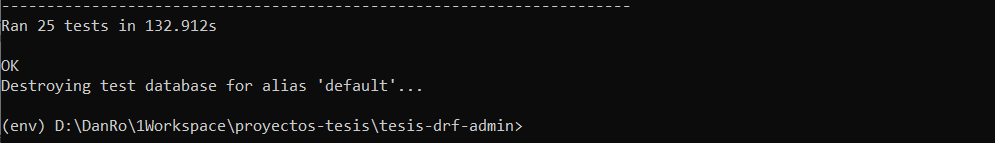
\includegraphics[width=0.9\textwidth]{images/TestCase.PNG} 
	\caption{Resultado de las pruebas unitarias.}
	\label{fig:unit_tests}
\end{figure}

\section{Pruebas funcionales}

Este tipo de prueba se realiza sobre el sistema funcionando, comprobando que cumpla con la especificación. Para estas pruebas, se utilizan las especificaciones de casos de prueba. Las pruebas basadas en requerimientos son pruebas de validación más que de defecto: se intenta demostrar que el sistema implementó adecuadamente sus requerimientos~\cite{sommerville2011software}.

\subsection{Método de caja negra}
Las pruebas de caja negra, también llamadas pruebas de comportamiento, se enfocan en los requerimientos funcionales del software. Las técnicas de prueba de caja negra permiten derivar conjuntos de condiciones de entrada que revisarán los requerimientos funcionales para un programa~\cite{pressman2010practitioner}. El método de caja negra presenta varias técnicas de prueba como son: partición de equivalencia y análisis de valores límites.
En la presente investigación se utilizará específicamente dentro del método de caja negra la técnica de partición de equivalencia generando los casos de pruebas de dicha técnica
sobre las diferentes interfaces que responden a los requisitos funcionales. Para la aplicación de pruebas de regresión sobre los casos de prueba definidos se usará la herramienta \textit{Selenium IDE} (Figura \ref{fig:unit_test}), que permite grabar todas las interacciones de un usuario con el navegador y posibilita ejecutar de forma automática las mismas, reduciendo el tiempo y los costos de las pruebas funcionales.

\begin{figure}[htbp] % h: here, t: top, b: bottom, p: page of floats - ajusta según necesidad
	\centering
	% Asegúrate de que la ruta 'images/arquitectura_web.png' sea correcta
	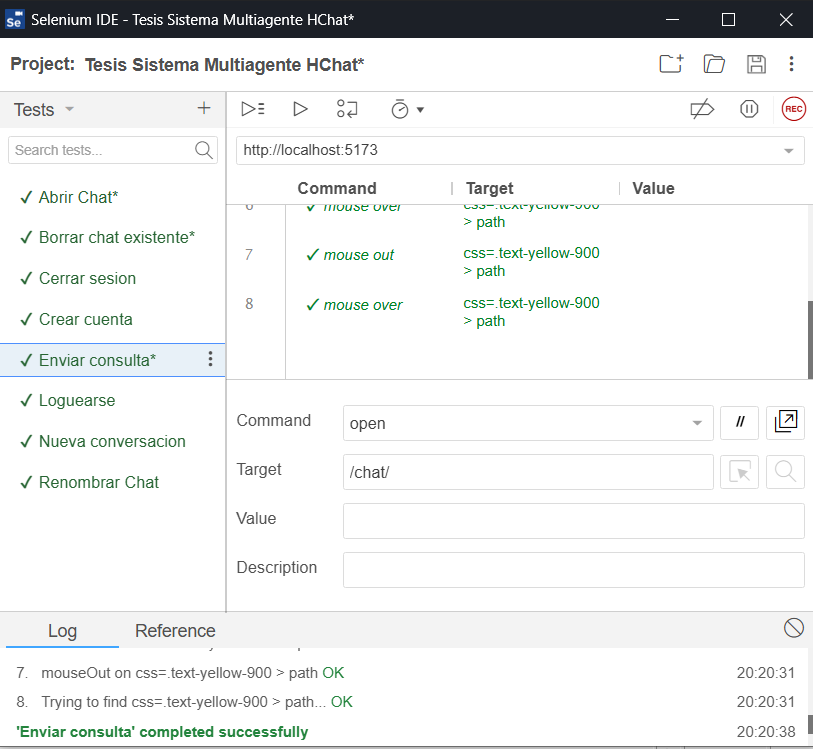
\includegraphics[width=0.42\textwidth]{images/Pruebas_funcionales.PNG} 
	\caption{Representación del resultado la ejecución de una prueba usando Selenium IDE, del requisito Insertar consulta.}
	\label{fig:unit_test}
\end{figure}

A continuación, la Tabla \ref{tab:caso_prueba_enviar_consulta}  muestra el diseño de caso de pruebas del requisito “Insertar consulta” donde se analizarán las variables y condiciones que puedan determinar la respuesta del sistema.


\begin{small} 
	\begin{longtable}{|p{2.2cm}|p{3cm}|p{3.2cm}|p{3.2cm}|p{3.2cm}|}
		\caption{Caso de prueba para la funcionalidad Insertar Consulta (Fuente: Elaboración Propia).} \label{tab:caso_prueba_enviar_consulta} \\
		\hline
		\textbf{Escenario} & \textbf{Descripción} & \textbf{Variables (Mensaje)} & \textbf{Respuesta Esperada} & \textbf{Respuesta} \\
		\hline
		\endfirsthead
		
		\hline
		\textbf{Escenario} & \textbf{Descripción} & \textbf{Variables (Consulta)} & \textbf{Respuesta Esperada} & \textbf{Respuesta} \\
		\hline
		\endhead
		
		\hline
		\endfoot
		
		\hline
		\endlastfoot
		
		EC 1.1. Enviar consulta correctamente. & El usuario debe escribir la consulta y dar clic en el botón de enviar. & ¿Cuantos barcos entraron al puerto de La Habana en 1851? & 567 & 567 \\
		\hline
		EC 1.2. Enviar consulta incorrecta(con un contexto fuera de la información conocida por el sistema). & El usuario debe escribir la consulta y dar clic en el botón de enviar. & ¿Cuánto tiempo duró la 2da guerra mundial? & Lo lamento no tengo esa información disponible. & La información solicitada no se encuentra. Por favor reformule la consulta. \\
		\hline
		EC 1.3. Solicitar un consulta cuya respuesta sea una gráfica. & El usuario debe escribir la consulta y dar clic en el botón de enviar. & Genera una gráfica con el \% de los barcos que entraron a La Habana con arroz en diferentes años. & La respuesta debe ser una gráfica. & Responde con una gráfica correspondiente acorde a la consulta. \\
		\hline
		\hline
		EC 1.4. Enviar consulta vacía & El usuario debe dar clic en el botón de enviar. & - & No se efectúa el envió de consultas vacías. & No se envía la consulta vacía. \\
		\hline
		
	\end{longtable}
\end{small}

\begin{table}[H]
	\caption{Variables de caso de prueba “Insertar Consulta” (Fuente: Elaboración Propia).}
	\label{tab:variables_insertar_consulta}
	\centering
	\begin{tabular}{|c|c|c|p{8.5cm}|}
		\hline
		\textbf{No.} & \textbf{Variable} & \textbf{Valor Nulo} & \textbf{Descripción} \\
		\hline
		1 & Consulta & No & Es un campo de texto que permite al usuario escribir una consulta al sistema \\
		\hline
	\end{tabular}
	
\end{table}

Las pruebas de caja negra se aplicaron con el objetivo de evaluar las interfaces de comunicación con el
usuario, las que demostraron coherencia y funcionalidad, así como probar todas aquellas funcionalidades
directamente relacionadas con los requisitos funcionales del sistema. La técnica de partición de equivalencia
es aplicada para evaluar los diferentes escenarios que pueden tener lugar ante la ejecución de una acción.
Como resultado de la aplicación de estas pruebas se ejecutan las posibles variantes que posee una interfaz
de comunicación con el usuario, resolviendo las no conformidades arrojadas y perfeccionando lo obtenido.

En este proceso se evaluaron las distintas variantes de la interfaz de comunicación con el usuario, permitiendo identificar y corregir no conformidades, así como perfeccionar la solución propuesta. Durante el proceso de pruebas se ejecutaron un total de 8 casos de prueba y tres iteraciones de prueba. En la primera iteración se identificaron 5 no conformidades, clasificadas en dos categorías: de funcionalidad y validación de datos. En la segunda iteración, mediante pruebas de regresión automatizadas con \textit{Selenium IDE}, se comprobó la corrección de las no conformidades detectados previamente, aunque surgieron 2 nuevas no conformidades relacionadas únicamente con la validación. Finalmente, en la tercera iteración no se detectaron nuevas no conformidades, cumpliéndose satisfactoriamente los requisitos funcionales definidos. La Figura \ref{fig:grafica_rf} ilustra la evolución de los resultados obtenidos en cada iteración.
\begin{figure}[htbp] % h: here, t: top, b: bottom, p: page of floats - ajusta según necesidad
	\centering
	% Asegúrate de que la ruta 'images/arquitectura_web.png' sea correcta
	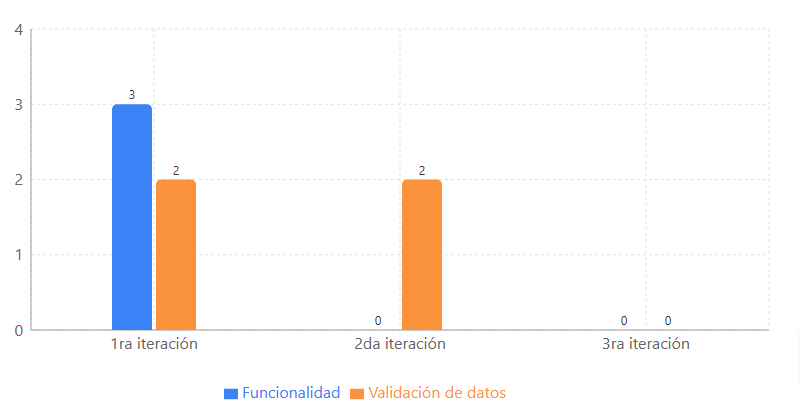
\includegraphics[width=0.5\textwidth]{images/grafica_pruebas_funcionales.PNG} 
	\caption{Representación del resultado de las pruebas funcionales (Fuente: Elaboración Propia).}
	\label{fig:grafica_rf}
\end{figure}



\section{Pruebas de rendimiento}

Las pruebas de rendimiento deben diseñarse para garantizar que el sistema procese su carga pretendida. Esto
implica efectuar una serie de pruebas donde se aumenta la carga, hasta que el rendimiento del sistema se
vuelve inaceptable. Las pruebas de rendimiento se preocupan tanto por demostrar que el sistema cumple
con sus requerimientos, como por descubrir problemas y defectos en el sistema~\cite{sommerville2011software}.

Para la realización de las pruebas de rendimiento del sistema se utilizó la herramienta Locust destinada para
la ejecución de estas pruebas mediante código python. La cuál permitió probar la aplicación simulando un
entorno similar al de producción, donde actuaban de forma concurrente 20 usuarios, realizando alrededor de 5 peticiones por segundo, obteniendo un tiempo de respuesta máximo
menor que cinco segundos y en el punto final más critico del sistema se obtuvo para el 95\% de los casos un tiempo de respuesta promedio de 11 segundos, cumpliendo así con lo pactado con el cliente en los requisitos no funcionales del
sistema. Estos resultados se pueden apreciar en la Figura \ref{fig:rend1}. Es fundamental interpretar los resultados de las pruebas de rendimiento presentados anteriormente teniendo en cuenta las especificaciones del entorno de prueba y las características de los servicios externos involucrados, como el proveedor de Inteligencia Artificial.

Las pruebas de rendimiento se ejecutaron a la API Django operando en una máquina con las siguientes características:

\begin{itemize}
	\item \textbf{Procesador:} Intel(R) Core(TM) i7-2670QM CPU @ 2.20GHz
	\item \textbf{Velocidad Base del Procesador:} 2.20 GHz (2201 MHz)
	\item \textbf{Núcleos Físicos:} 4 procesadores principales
	\item \textbf{Procesadores Lógicos (Hilos):} 8 procesadores lógicos
\end{itemize}

Para la generación de respuestas por IA, la aplicación se integró con el servicio Google Gemini a través de su API. Esto implica que cada vez que se requiere una respuesta de la IA se envía una solicitud a la API de Gemini~\footnote{La API de Google Gemini es una interfaz desarrollada por Google que permite integrar en tus aplicaciones los modelos de inteligencia artificial generativa más avanzados de Google, conocidos como Gemini. Estos modelos son nativos multimodales: pueden procesar y generar respuestas a partir de texto, imágenes, audio, video y documentos no estructurados como PDFs.} que tiene tiempos de respuestas de mayor velocidad que si se utiliza un modelo en local. Los resultados actuales deben considerarse como una línea base específica para este entorno y esta configuración de IA. Es altamente probable que las métricas de rendimiento cambien (y potencialmente mejoren significativamente) bajo otras circunstancias donde se cuente con mayor cantidad de RAM~\footnote{La RAM (Memoria de Acceso Aleatorio, o Random Access Memory en inglés) es un tipo de memoria principal que utiliza tu computadora, teléfono móvil u otros dispositivos para almacenar temporalmente los datos y programas que se están utilizando en ese momento.}, mejor procesador y almacenamiento SSD~\footnote{El almacenamiento SSD (\textit{Solid State Drive} o unidad de estado sólido) es un dispositivo de almacenamiento de datos que utiliza memoria flash para almacenar información, a diferencia de los discos duros tradicionales (HDD), que usan discos magnéticos y partes móviles.}.\\

\begin{figure}[htbp] % h: here, t: top, b: bottom, p: page of floats - ajusta según necesidad
	\centering
	% Asegúrate de que la ruta 'images/arquitectura_web.png' sea correcta
	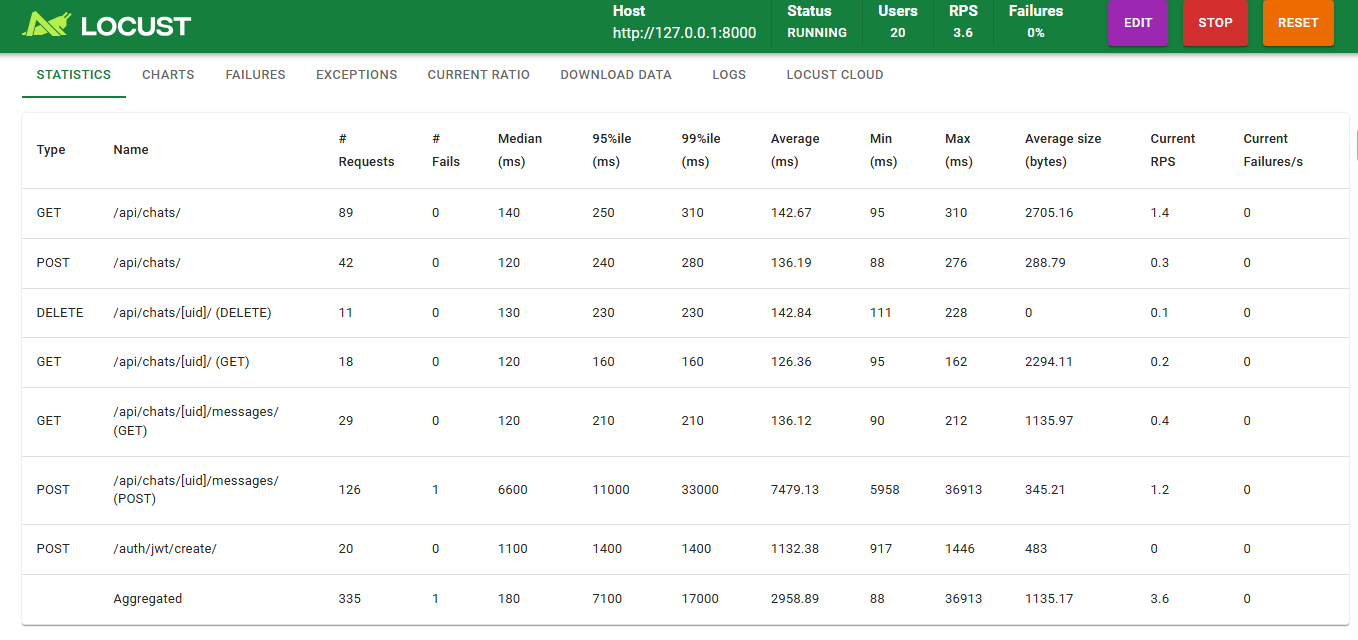
\includegraphics[width=0.9\textwidth]{images/Rendimiento1.PNG} 
	\caption{ Prueba de rendimiento en Locust}
	\label{fig:rend1}
\end{figure}

\section{Pruebas de seguridad}

Las pruebas de seguridad se diseñan para sondear las vulnerabilidades del entorno del lado del cliente, las
comunicaciones de red que ocurren conforme los datos pasan de cliente a servidor y viceversa, y el entorno
del lado servidor. Cada uno de estos dominios puede atacarse, y es tarea del examinador de seguridad
descubrir las debilidades que puedan explotar quienes tengan intención de hacerlo~\cite{pressman2010practitioner}.

Las pruebas de seguridad se aplicaron con ayuda de la herramienta Acunetix Web Vulnerability Scanner 9.5
que establece alertas de tipo: alta, media, baja e informacional, realizándose en dos iteraciones durante el
desarrollo de la propuesta solución.
En una primera iteración se obtuvo un total de 22 alertas de seguridad, de las cuales 4 clasifican de nivel
medio, 1 de nivel bajo y 17 informativas.

De las de nivel medio, se destacaron el uso de protocolo no seguro
para el envío de datos, así como los mensajes de error que se muestra en el modo DEBUG de Django para
el desarrollo y se detectaron problemas para la protección de contra ataques de fuerza bruta en el formulario
de autenticación.\\
La de nivel bajo, consistía en vistas del sitio que se podían acceder directamente sin pasar la autenticación
y el sistema de roles establecido. De carácter informativo fueron detectadas posibles cuentas de usuario en ficheros, así como presencia de directorios desprotegidos y la existencia de etiquetas iframe de HTML5.

Después de aplicar refactorización del código y realizar las validaciones correspondientes, se aplicó la segunda iteración en búsqueda de vulnerabilidades al sistema, arrojando como resultado que todas las que se habían detectado en la primera iteración, habían sido corregidas.

Resultados de las iteraciones: 

\begin{figure}[htbp] % h: here, t: top, b: bottom, p: page of floats - ajusta según necesidad
	\centering
	% Asegúrate de que la ruta 'images/arquitectura_web.png' sea correcta
	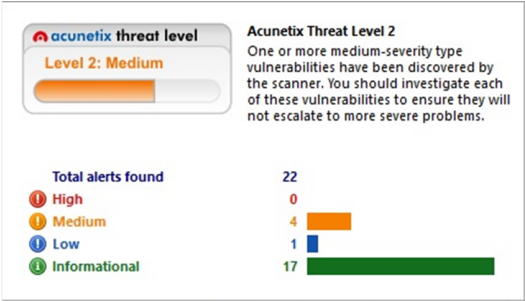
\includegraphics[width=0.5\textwidth]{images/primeraIt.PNG} 
	\caption{ Prueba de seguridad 1ra iteración.}
	\label{fig:grafica_segur}
\end{figure}

\begin{figure}[htbp] % h: here, t: top, b: bottom, p: page of floats - ajusta según necesidad
	\centering
	% Asegúrate de que la ruta 'images/arquitectura_web.png' sea correcta
	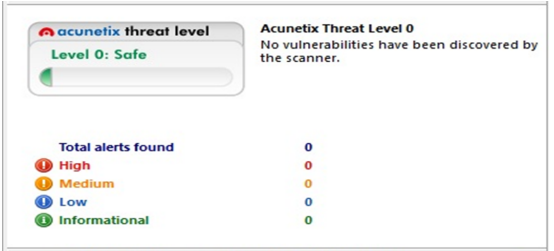
\includegraphics[width=0.5\textwidth]{images/2iter.PNG} 
	\caption{ Prueba de seguridad 2da iteración.}
	\label{fig:grafica_segu2}
\end{figure}

%\section{Pruebas de aceptación}
%\label{sec:pruebas-aceptacion}

%Las pruebas de aceptación, también conocidas como pruebas de usuario, constituyen la fase final de verificación antes de la entrega o despliegue del software. Su objetivo principal es validar que el sistema cumple con las necesidades y expectativas del cliente o usuario final, y que es apto para su propósito en el entorno operativo real o simulado~\cite{pressman2010practitioner}. Estas pruebas se realizan desde la perspectiva del usuario, enfocándose en la funcionalidad global y la usabilidad del sistema, en lugar de en los detalles técnicos internos.

%Para el sistema multiagente conversacional desarrollado, se planificaron \textbf{pruebas alfa} como principal método de prueba de aceptación. Este tipo de prueba implica la participación de un grupo selecto de usuarios finales o representantes del cliente (en este caso, podrían ser historiadores, investigadores o académicos interesados en el \textit{Diario de la Marina}), quienes interactúan con el sistema en un entorno controlado, usualmente el entorno de desarrollo o uno de staging muy similar al de producción.

%\textbf{Metodología de las Pruebas Alfa:}
%\begin{itemize}
	%\item \textbf{Selección de Participantes:} Se identificarán usuarios con conocimiento del dominio histórico del \textit{Diario de la Marina} y con diferentes niveles de familiaridad con herramientas tecnológicas.
	%\item \textbf{Definición de Escenarios de Uso:} Se prepararán escenarios de prueba basados en casos de uso reales y representativos, como la formulación de consultas históricas específicas, la solicitud de contextualización de eventos, y la interacción general con el asistente conversacional para explorar la información contenida en el periódico.
	%\item \textbf{Ejecución de Pruebas:} Los participantes utilizarán el sistema para completar los escenarios definidos. Se les alentará a explorar libremente y a registrar cualquier problema, duda, sugerencia o aspecto que consideren relevante.
	%\item \textbf{Recopilación de Feedback:} Se utilizarán cuestionarios, entrevistas y observación directa para recopilar la retroalimentación de los participantes. Se prestará especial atención a:
	%\begin{itemize}
		%\item Facilidad de uso de la interfaz.
		%\item Claridad y precisión de las respuestas generadas por el sistema.
		%\item Relevancia y contextualización de la información recuperada.
		%\item Satisfacción general con la interacción.
		%\item Identificación de posibles errores funcionales o comportamientos inesperados no detectados en fases anteriores.
	%\end{itemize}
	%\item \textbf{Análisis de Resultados:} La retroalimentación recopilada será analizada para identificar patrones, problemas recurrentes y áreas de mejora. Estos hallazgos servirán para realizar ajustes finales al sistema antes de su posible despliegue o para planificar futuras iteraciones de desarrollo.
%\end{itemize}

%El objetivo de estas pruebas de aceptación no es solo confirmar que el sistema "funciona", sino asegurar que realmente aporta valor al usuario final y que su integración en un flujo de trabajo de investigación histórica sería beneficiosa y eficiente. La validación por parte de los usuarios clave es crucial para el éxito y la adopción del sistema multiagente conversacional.

%Como resultado de haber aplicado las pruebas alfa se identificaron tres nuevas no conformidades las cuales fueron resueltas en su totalidad.

% (Opcional: Si ya se realizaron algunas pruebas alfa y tienes resultados preliminares, podrías añadir un breve párrafo aquí. Si no, puedes dejarlo como la planificación).
% Ejemplo si tienes resultados:
% "En una fase preliminar de pruebas alfa con un grupo reducido de X investigadores, se observó una recepción generalmente positiva hacia la capacidad del sistema para [mencionar un logro clave]. Sin embargo, se identificaron áreas de mejora en [mencionar un área], las cuales serán abordadas en futuras iteraciones."

%\subsection{Satisfacción de los usuarios}

%\begin{table}[htbp]
%	\caption{Cuadro Lógico de Iadov para la Evaluación del Sistema Multiagente Conversacional (Fuente: Elaboración propia).}
%	\label{tab:cuadro-iadov-foto} % Nueva etiqueta para esta tabla de imagen
%	\centering
%	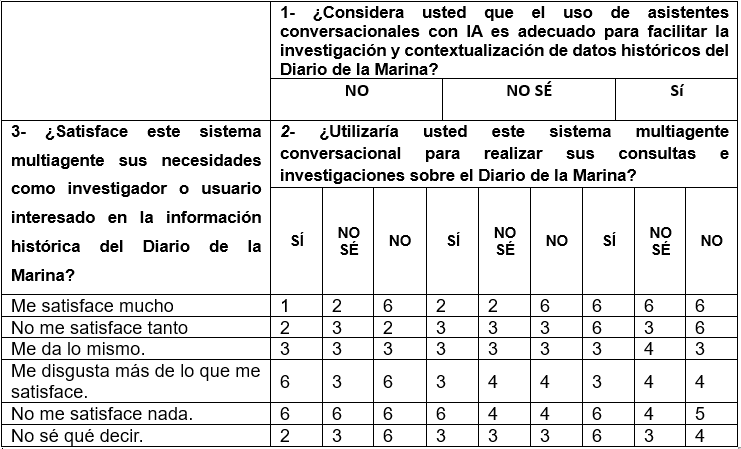
\includegraphics[width=0.8\textwidth]{images/Tabla de iadov.PNG}\\
%\end{table}

%Con el objetivo de evaluar el sistema implementado se utiliza la técnica de Iadov, esta técnica evalúa el nivel de satisfacción del usuario, permitiendo conocer si la solución propuesta cumple con las expectativas esperadas. Esta técnica constituye una vía indirecta para el estudio de la satisfacción, ya que los criterios que se utilizan se fundamentan en las relaciones que se establecen entre tres preguntas cerradas (preguntas 1, 2 y 3) que se intercalan dentro de un cuestionario (Ver \textbf{Anexo C})~\cite{tinajero2021tecnica}. Estas tres preguntas se relacionan a través de lo que se denomina el “Cuadro Lógico de Iadov”, el cual se muestra a continuación en la Tabla \ref{tab:cuadro-iadov-foto}.

%El número resultante de la interrelación de las tres preguntas indica la posición de cada sujeto en la escala de satisfacción individual y grupal.


\section*{Conclusiones del capítulo}
\addcontentsline{toc}{section}{Conclusiones del Capítulo}
\label{sec:conclusiones-cap3}

La fase de pruebas del sistema multiagente conversacional ha proporcionado una validación integral de su funcionalidad y rendimiento, arrojando resultados significativos sobre su estado actual y áreas de potencial optimización como son la latencia de respuesta y la mejora de su contextualización.

Los componentes individuales del sistema demostraron una alta fiabilidad a nivel unitario, superando con éxito un total de 25 casos de prueba automatizados, incluyendo aquellos diseñados con la técnica del camino básico para requisitos funcionales críticos, sin registrarse errores tras las correcciones pertinentes. Esto subraya la robustez interna del código desarrollado.

Desde la perspectiva funcional, el sistema cumplió con el 100\% de los requisitos especificados. Las pruebas de caja negra, iteradas hasta la corrección de todas las no conformidades identificadas, confirmaron que las interacciones del usuario y las respuestas del sistema se comportan según lo esperado, validando la correcta implementación de las funcionalidades de cara al usuario.

Las pruebas de rendimiento, ejecutadas con \textit{Locust} bajo una carga de 20 usuarios concurrentes, indicaron que la mayoría de los \textit{endpoints} de la \textit{API} operan con tiempos de respuesta eficientes (inferiores a 5 segundos), el \textit{endpoint} de envío de mensajes y generación de respuesta por IA (\textit{`POST /api/chats/[uid]/messages/`}) presenta una latencia considerable, con un tiempo de respuesta promedio para el 95\% de los casos de 11 segundos debido a su alta complejidad y dependencia del microservicio del sistema multiagente.

En el ámbito de la seguridad, el análisis mediante \textit{Acunetix Web Vulnerability Scanner} reveló y permitió subsanar vulnerabilidades de nivel medio y bajo en una primera iteración, incluyendo la protección contra ataques comunes y la corrección de configuraciones inseguras. La segunda iteración de pruebas confirmó la efectividad de estas mitigaciones, resultando en un sistema sin alertas de seguridad críticas.  

En síntesis, las pruebas realizadas confirman que el sistema multiagente es funcionalmente completo, seguro contra las vulnerabilidades evaluadas y cumple con los umbrales de rendimiento establecidos, al tiempo que señalan la interacción con la IA como un área prioritaria para futuras optimizaciones enfocadas en la escalabilidad y la mejora de la experiencia de usuario en tiempo real.